\chapter{Antes de empezar}

Hay que tener en cuenta que lo que se va a explicar en este documento es el acceso a AWS Academy, por lo que existe una pequeña diferencia con una cuenta de AWS estándar, como la que se obtendría al crear una cuenta real y al introducir los datos de la tarjeta de crédito.

\href{https://aws.amazon.com/es/training/awsacademy/}{AWS Academy} ofrece a las instituciones de educación superior un plan de estudios de computación en la nube gratuito y la posibilidad de crear laboratorios personalizados, o libres, para poder realizar despliegues en un sistema de nube pública.

La ventaja de AWS Academy es que va a permitir a los alumnos a hacer uso del interfaz y de la infraestructura de AWS sin tener que hacer uso de una tarjeta de crédito. Ahora bien, \textbf{existen ciertas limitaciones} que no nos encontraríamos en una cuenta de AWS real.

Como vamos a hacer uso de la infraestructura real de AWS, para que no se abuse de ello, los laboratorios estarán limitados a una cantidad de 100\$ y de 4 horas de uso límite. A medida que vamos realizando despliegues o vamos utilizando servicios, la cantidad de dinero irá disminuyendo.

Por otro lado, para evitar que los servicios se queden corriendo (y por tanto, gasten dinero), los laboratorios tendrán un contador que al llegar a 4 horas se apagarán. \textbf{No existe problema en volver a iniciar el laboratorio, o resetear el contador}.


\chapter{Acceder a los cursos}

Para acceder a los cursos en los que el profesor nos ha matriculado, nos habrá llegado un mail que nos mandará a una página donde tendremos que indicar si tenemos ya una cuenta o tenemos que crearla:

\begin{center}
	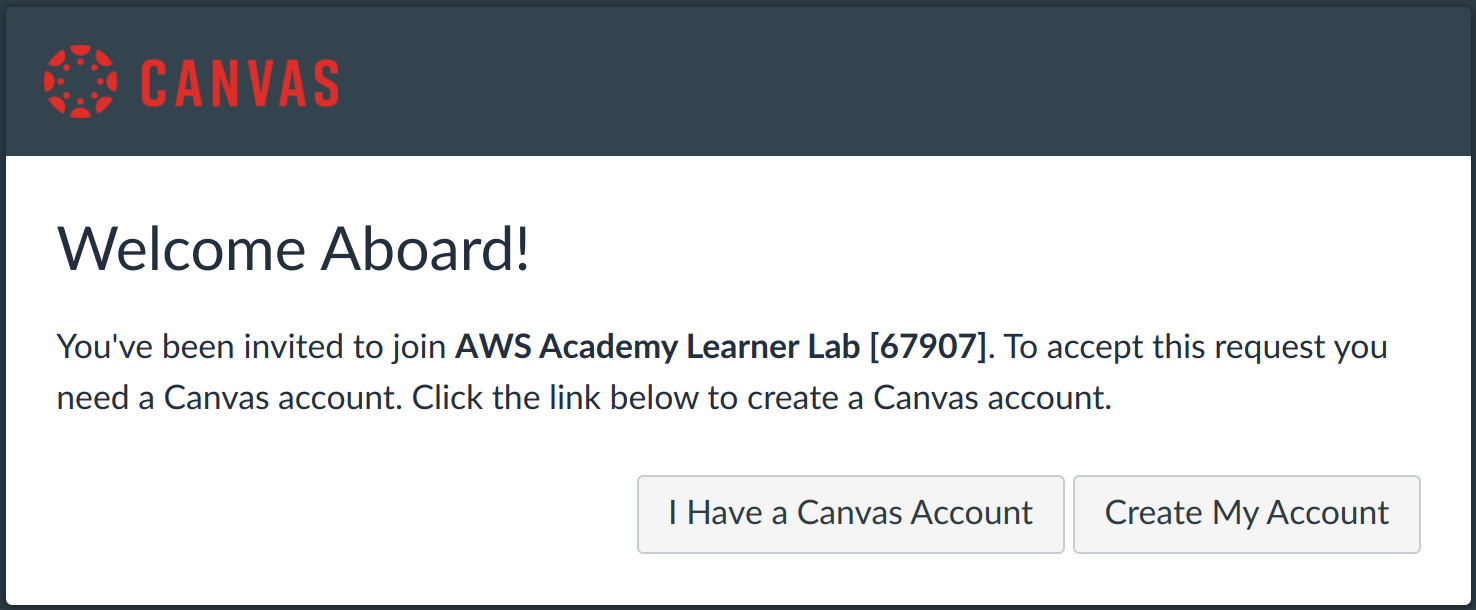
\includegraphics[width=0.7\linewidth]{img/aws/create_account.png}
\end{center}

Debemos introducir una contraseña y aceptar los terminos para poder crear la cuenta. Una vez creada, nos mandará directamente al curso al que nos han matriculado.

Si ya tenemos una cuenta creada previamente, podemos ir al \href{https://www.awsacademy.com/vforcesite/LMS_Login}{panel de acceso} y elegir la opción \textbf{Student Login}. En ese punto nos aparecerá el formulario en el que debemos introducir el nombre de usuario y la contraseña.

\begin{center}
	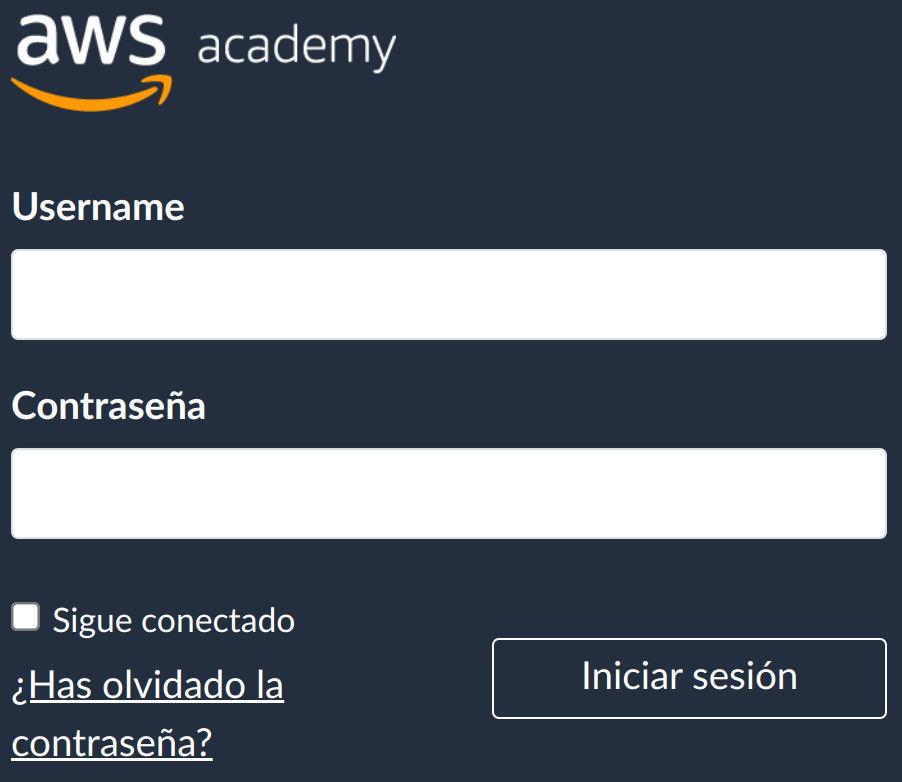
\includegraphics[width=0.5\linewidth]{img/aws/login.png}
\end{center}

\chapter{Acceder al laboratorio}

Una vez logueado veremos los posibles cursos en los que estamos matriculados, y debemos ir al curso correspondiente. Una vez en el curso, luego hay que ir a “Módulos → Iniciar el Laboratorio de aprendizaje de AWS Academy”, y aparecerá una página en el que abajo del todo tendréis un botón para aceptar las condiciones de uso, y luego veremos algo similar a la siguiente pantalla:

\begin{center}
	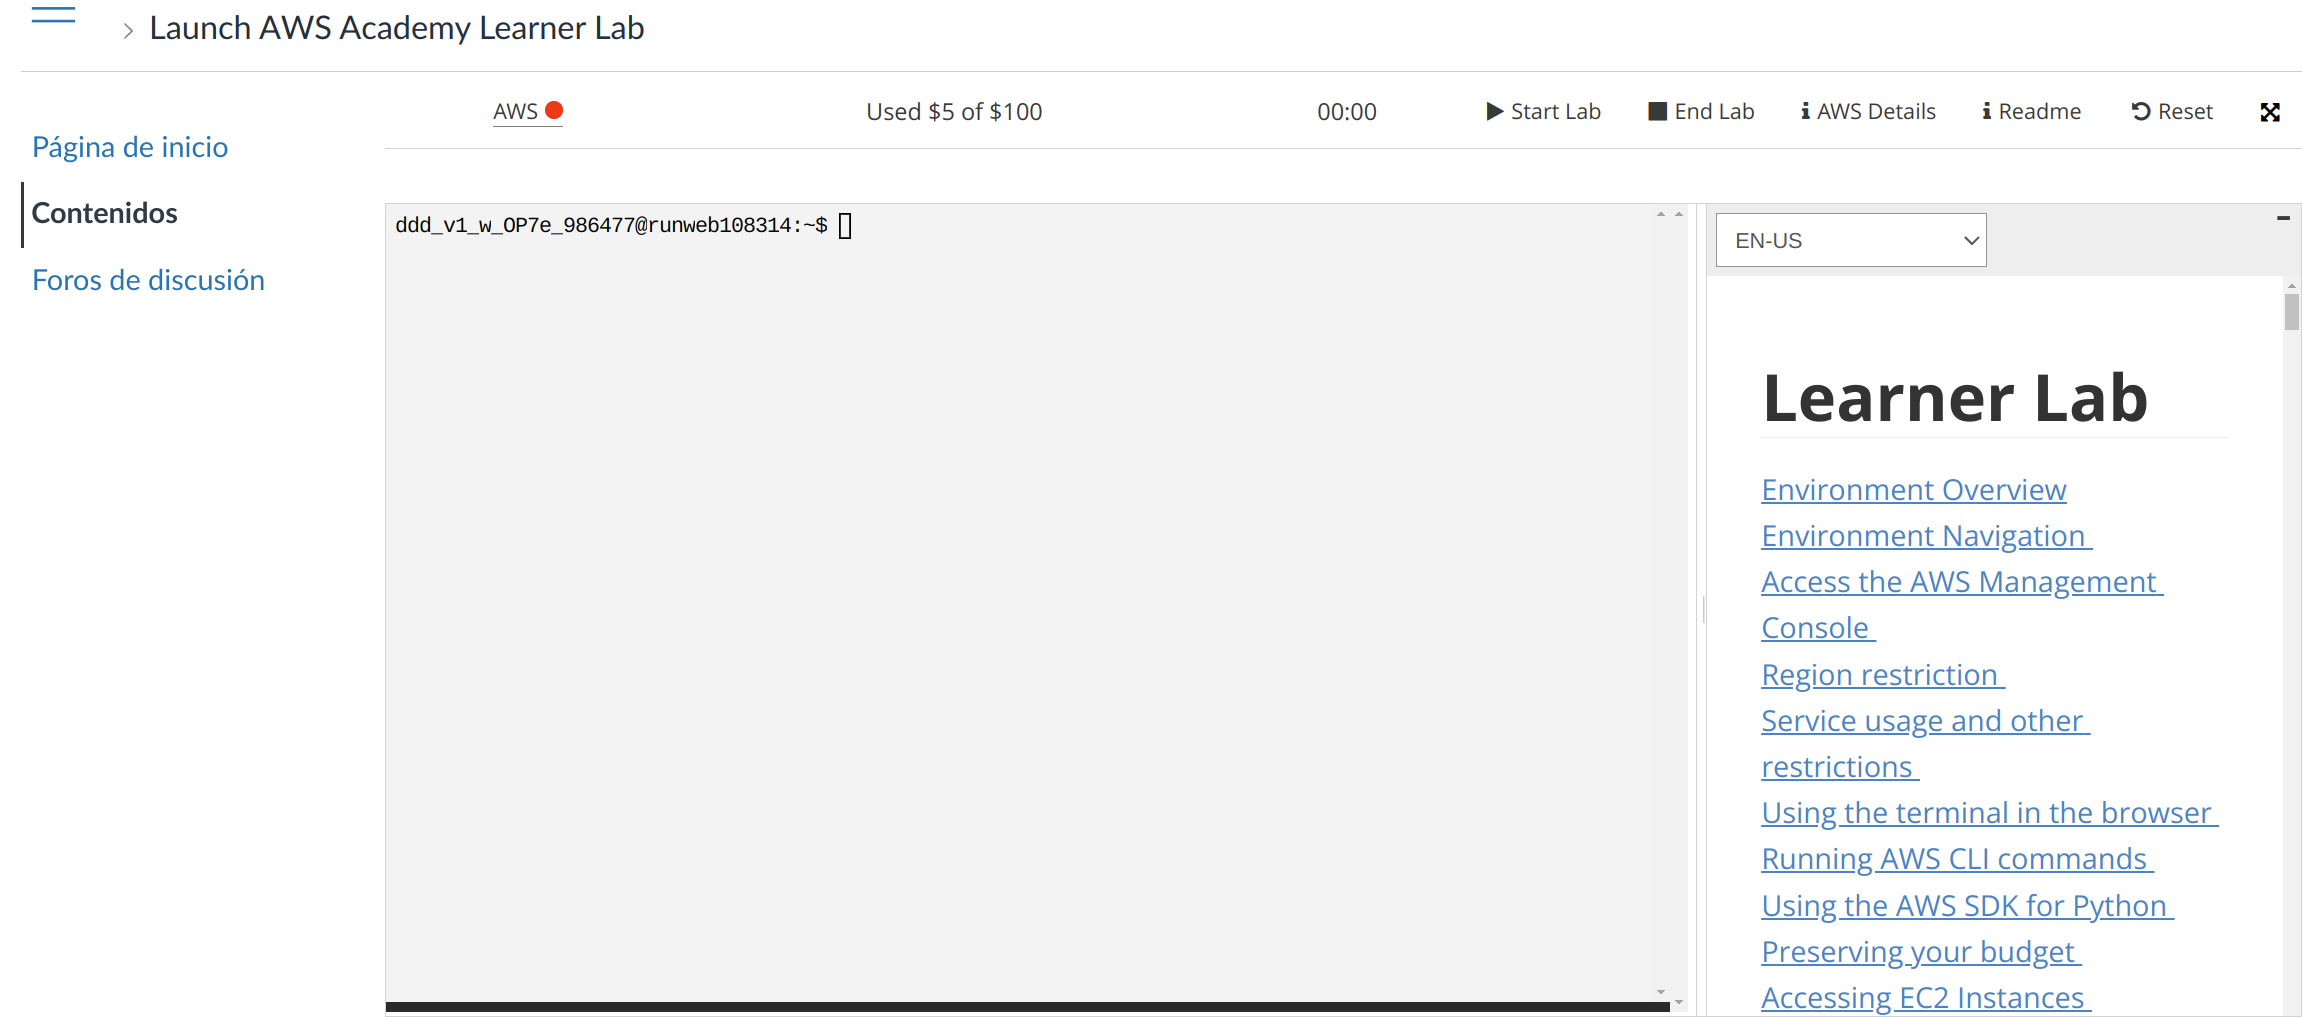
\includegraphics[frame, width=0.9\linewidth]{img/aws/launcher.png}
\end{center}

En esta pantalla podemos ver distinta información del propio laboratorio y su estado:

\begin{itemize}
	\item \textbf{AWS \color{red}●}: Estado visual del laboratorio. En este caso, el círculo aparece en rojo porque el laboratorio está apagado. Al darle a iniciar, se pondrá en color amarillo ({\color{yellow}●}) mientras el laboratorio se está preparando. Cuando esté listo para ser utilizado se pondrá en verde ({\color{green}●}).
	
	\item \textbf{Used \$5 of \$100}: Cuánto dinero nos hemos gastado en el laboratorio de los 100 dólares que tenemos. Este gasto no se actualiza en tiempo real, y pueden pasar algunas horas hasta que se refleje el gasto real.
	
	\item \textbf{00:00}: El tiempo que le queda al laboratorio encendido. Es una cuenta atrás de 4 horas. 
	
	\item \faPlay  \textbf{ Start Lab}: Iniciar el laboratorio.
	
	\item \faStop  \textbf{ End Lab}: Parar el laboratorio. Todo lo realizado se para, pero hay ciertos servicios que se siguen cobrando (almacenamiento de ciertos espacios).
	
	\item \faInfo  \textbf{ AWS Details}: Detalles del laboratorio. \textbf{Más adelante hablaremos de este apartado}.
	
	\item \faInfo  \textbf{ Readme}: Tutoriales y manuales sobre el laboratorio.
	
	\item \faUndo \textbf{ Reset}: Resetea el laboratorio y borrará todo el contenido realizado. Lo deja como si estuviese recién inicializado.
\end{itemize}

El terminal que aparece es un interfaz de administración para el laboratorio, y desde el que podríamos realizar administración del laboratorio, o incluso levantar nuevos servicios a través del CLI \textbf{aws}. Por otro lado, no lo vamos a utilizar.

\warnbox{\textbf{La primera vez que encendamos el laboratorio puede tardar entre 2 y 5 minutos.}}

Cuando tenemos el laboratorio encendido la imagen será la siguiente

\begin{center}
	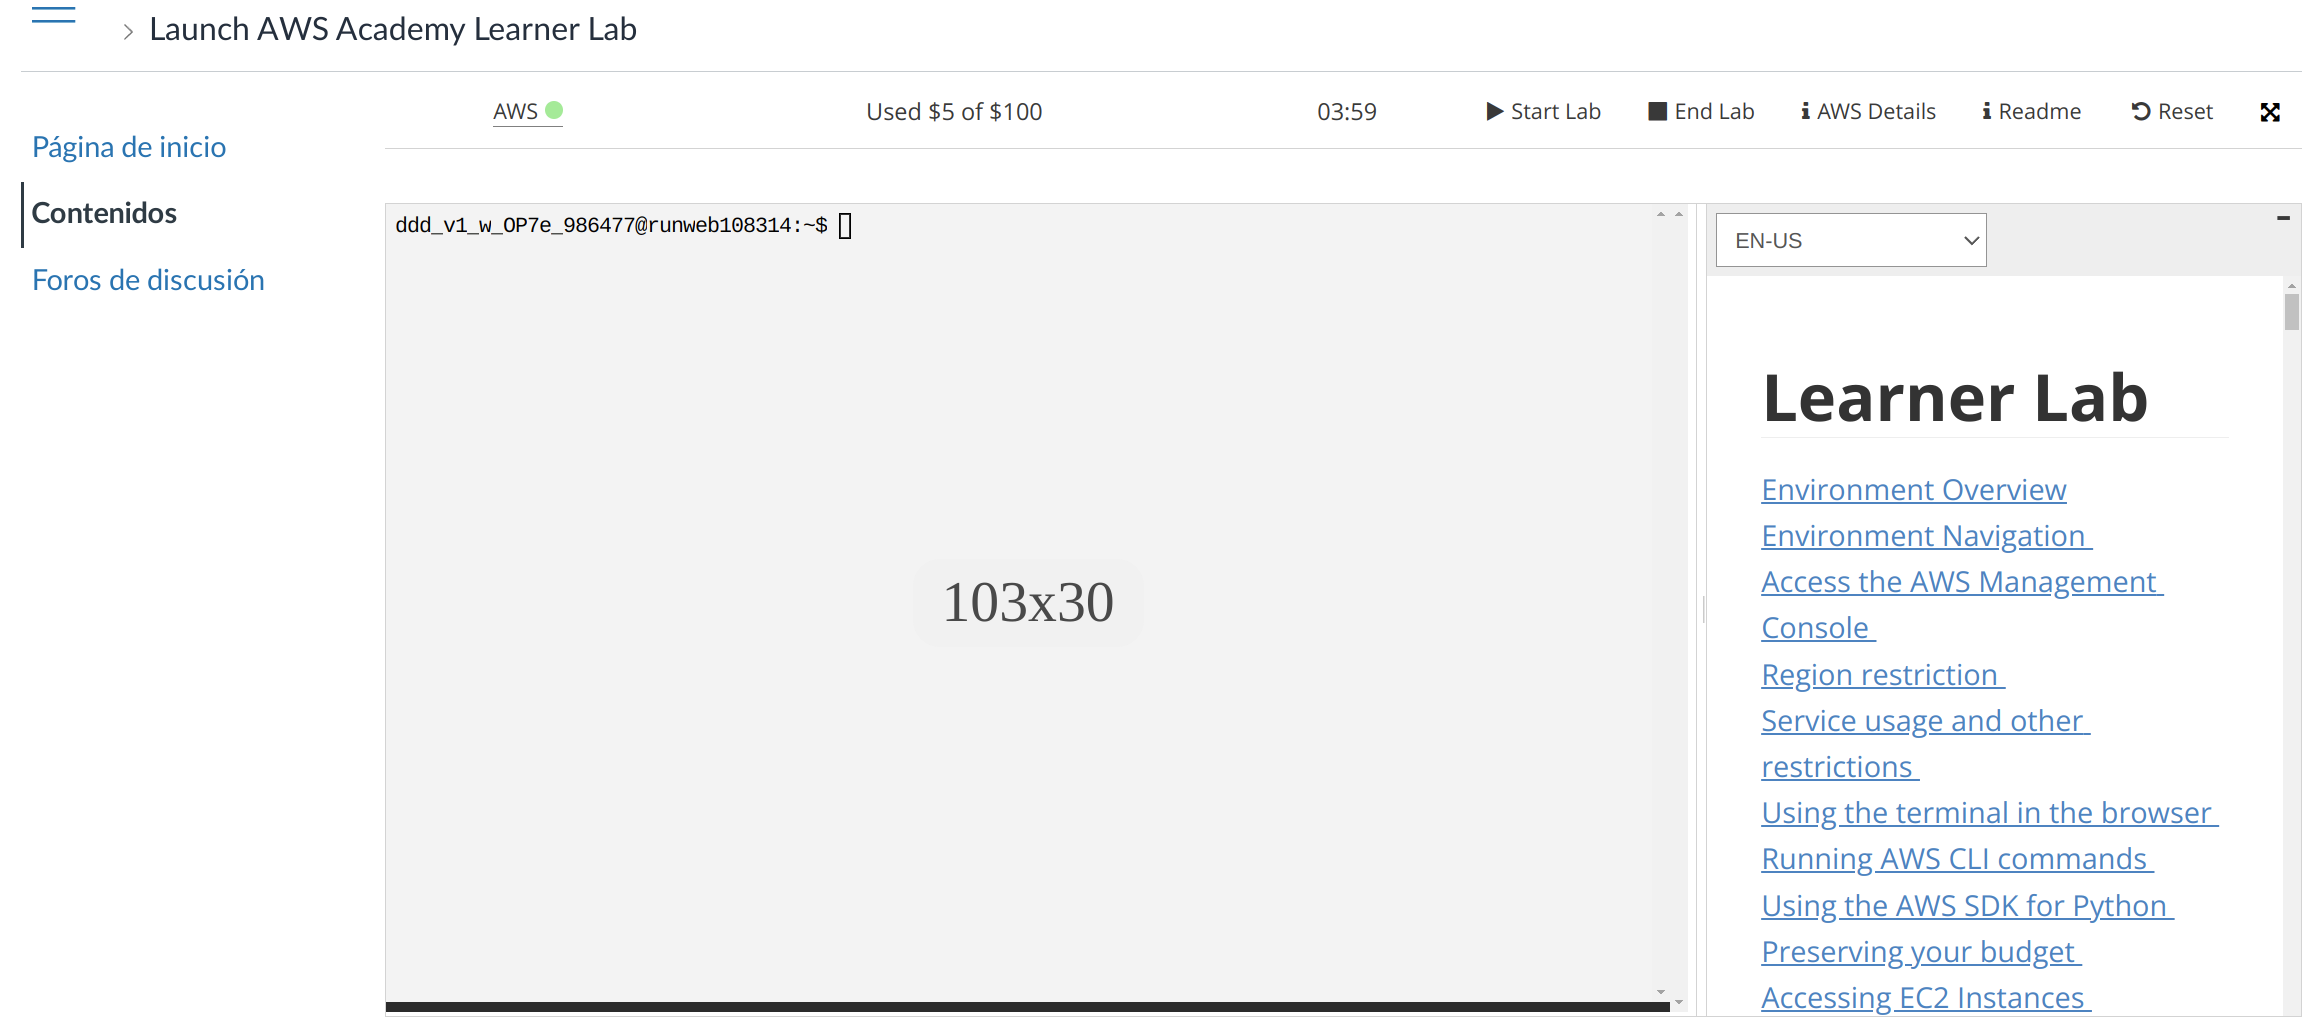
\includegraphics[frame, width=0.9\linewidth]{img/aws/launcher-started.png}
\end{center}

Para entrar en el laboratorio debemos hacer click en “{AWS \color{green}●}”, lo que nos abrirá una nueva pestaña en la que veremos el panel de administración (o “Consola” llamada por AWS) donde tendremos un resumen de los servicios que hemos visitado anteriormente, aplicaciones que tengamos desplegadas, coste... La idea es tener a simple vista lo que más estemos utilizando.


\chapter{Servicios básico de AWS}

AWS cuenta hoy en día con infinidad de servicios que podemos utilizar y desplegar. Es imposible abarcar todos en un curso, por lo que aprenderemos a utilizar y a entender sólo de unos pocos. Entre los que vamos a utilizar están:

\begin{itemize}
	\item \textbf{VPC}: Es la parte que nos proporciona la red virtual en la nube de Amazon, y todo lo que tiene que ver con direccionamiento de red, acceso a internet, ... 
	\item \textbf{EC2}: Parte central de AWS que se encarga de la computación virtual y otros servicios que tienen que ver con máquinas virtuales.
	\item \textbf{RDS}: Es el servicio para crear bases de datos relacionales de Amazon. Podemos crear servicios con distintos motores, con distinta configuración, escalado, ...
\end{itemize}

Cuando entremos a algunos de estos servicios, el interfaz web que nos vamos a encontrar, por norma general, suele ser muy parecido y tiene el siguiente aspecto:

\begin{center}
	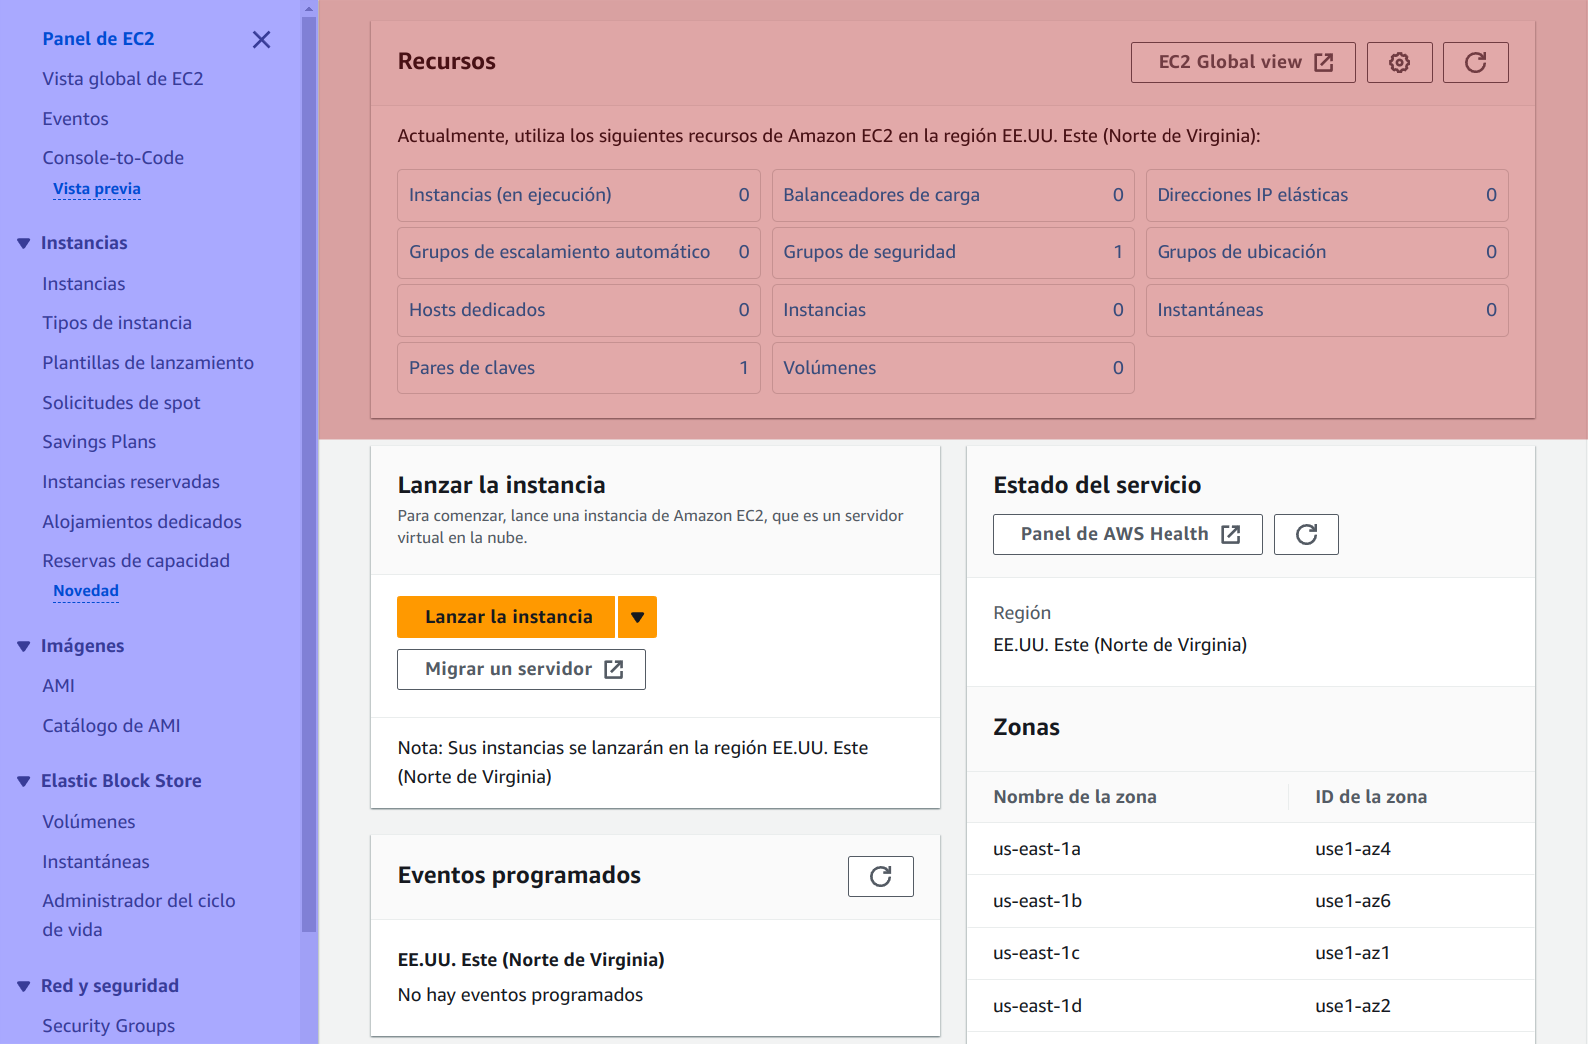
\includegraphics[width=0.8\linewidth]{img/aws/panel.png}
\end{center}

Podemos diferenciar dos apartados en la vista:
\begin{itemize}
	\item \textbf{Panel lateral izquierdo}: En la imagen resaltado de color azul, es un menú donde podemos ver distintos apartados diferenciados por grupos. Estos apartados nos permitirán crear o configurar servicios que se nos desplegarán en la vista principal.
	
	\item \textbf{Vista principal}: En este caso sólo se ha resaltado la parte superior, ya que al entrar a cada tipo de servicio, en esta parte aparece un resumen de los recursos que tenemos contratados.
	
	Esta vista central cambiará teniendo en cuenta la opción seleccionada del panel lateral.
\end{itemize}

\chapter{Regiones y zonas de disponibilidad}

Dado que AWS ofrece un servicio mundial, los servidores que nos ofrecen están desplegados a lo largo de distintos países, para que el acceso desde cada zona sea lo más rápida posible. Esta infraestructura global, actualmente está diferenciada de la siguiente manera tal como aparece en la \href{https://aws.amazon.com/es/about-aws/global-infrastructure/regions_az/?p=ngi&loc=2}{documentación oficial}:

\begin{center}
	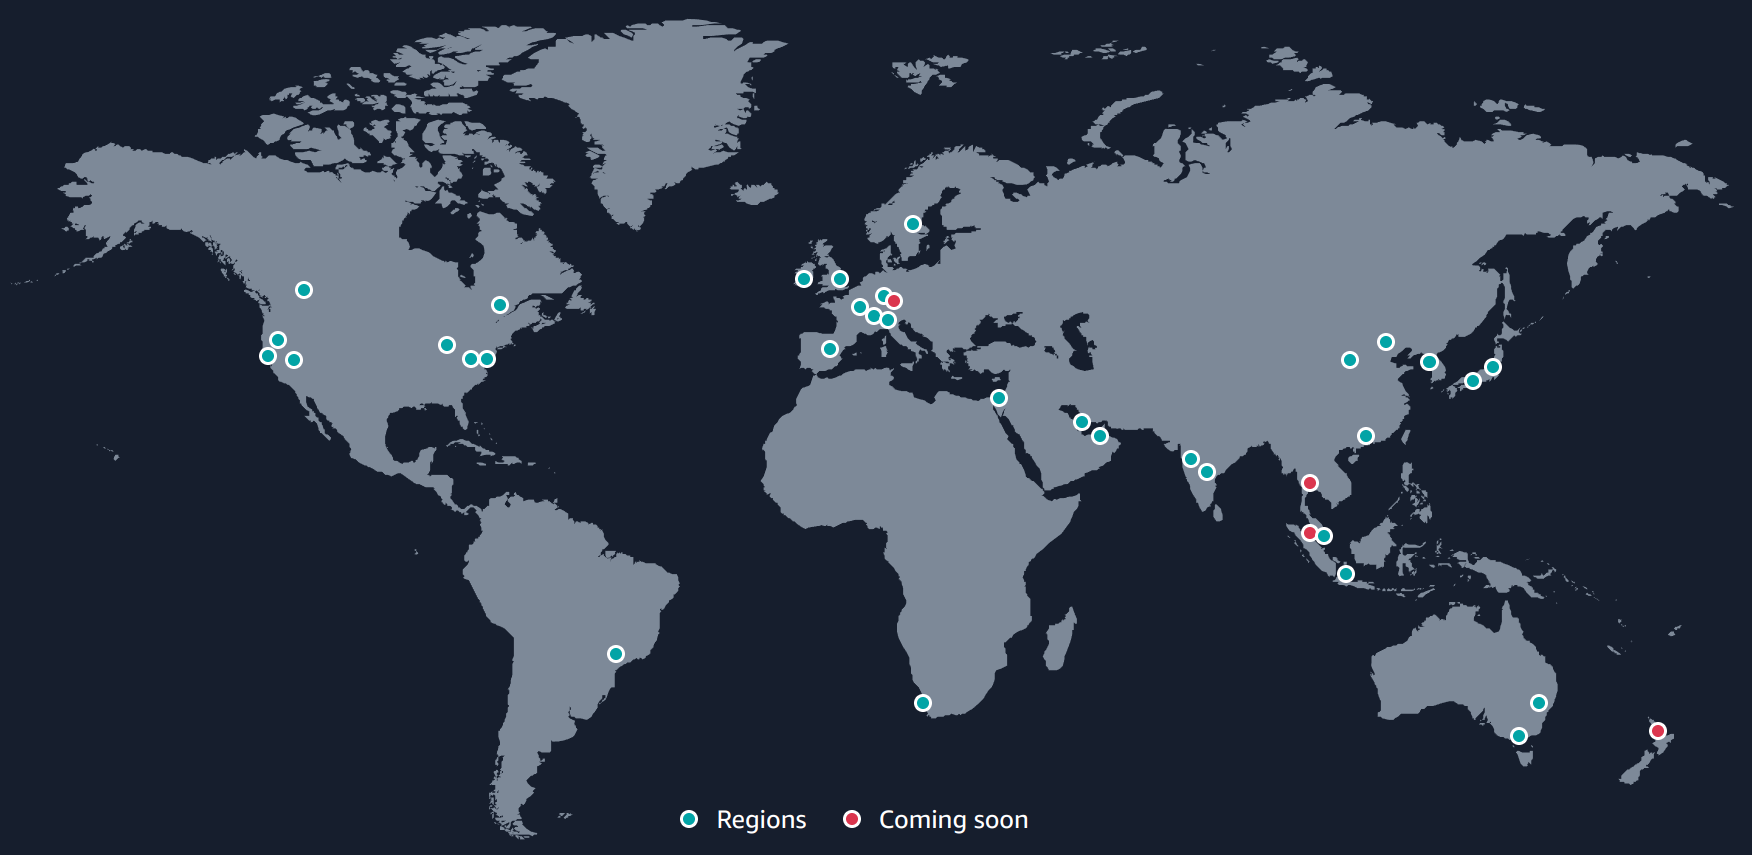
\includegraphics[width=0.8\linewidth]{img/aws/regiones.png}
\end{center}

\begin{itemize}
	\item \textbf{Regiones}: AWS tiene el concepto de una región, que es una ubicación física en todo el mundo donde se agrupan los centros de datos. Se llama a cada grupo de centros de datos lógicos “zona de disponibilidad”. 
	
	Ejemplo de Regiones en Europa: España (situada en Aragón), Irlanda, Fráncfort, Londres, París, Estocolmo, Milán, Zúrich.
	
	\item \textbf{Zonas de disponibildiad}: Cada región de AWS consta de un mínimo de tres zonas de disponibilidad con acceso aisladas y físicamente separadas dentro de un área geográfica. 
	
	El diseño múltiple de zonas de disponibilidad de cada región de AWS ofrece ventajas para los clientes. Cada zona de disponibilidad tiene alimentación, refrigeración y seguridad física independientes y está conectada a través de redes redundantes de latencia ultrabaja.
	
	
\end{itemize}

\warnbox{\textbf{AWS Academy está limitado sólo a la región “Norte de Virginia” de Estados Unidos.}}

Por limitaciones de AWS Academy, todo lo que creemos sólo va a ser creado en la regiónd “Norte de Virginia” de Estados Unidos. Esto puede hacer que haya algo más de latencia desde España, pero el resultado de aprendizaje será el mismo.
